\subsection{Macroeconomic Expectations}\label{subsec:macroExp}

We have identified only a few papers in macroeconomics (excluding finance; see above) that either constitute full-fledged EE modeling exercises or are closely related to such models. Figure~\ref{fig:graph_macro} depicts the network of citation connections between those papers.\footnote{See \dmwinflationexpectationFull, and \bvbayesianlearningFull, for non-social models of macroeconomic expectations formation.}

%\begin{center}[Insert Figure \ref{fig:graph_macro}  here]\end{center}


\begin{figure}[!ht] \centering  % [h!]
	%\hypertarget{graphmacro}{}
	\caption{ ~Literature map of EE models of macroeconomic expectations}
	\label{fig:graph_macro}
	\centerline{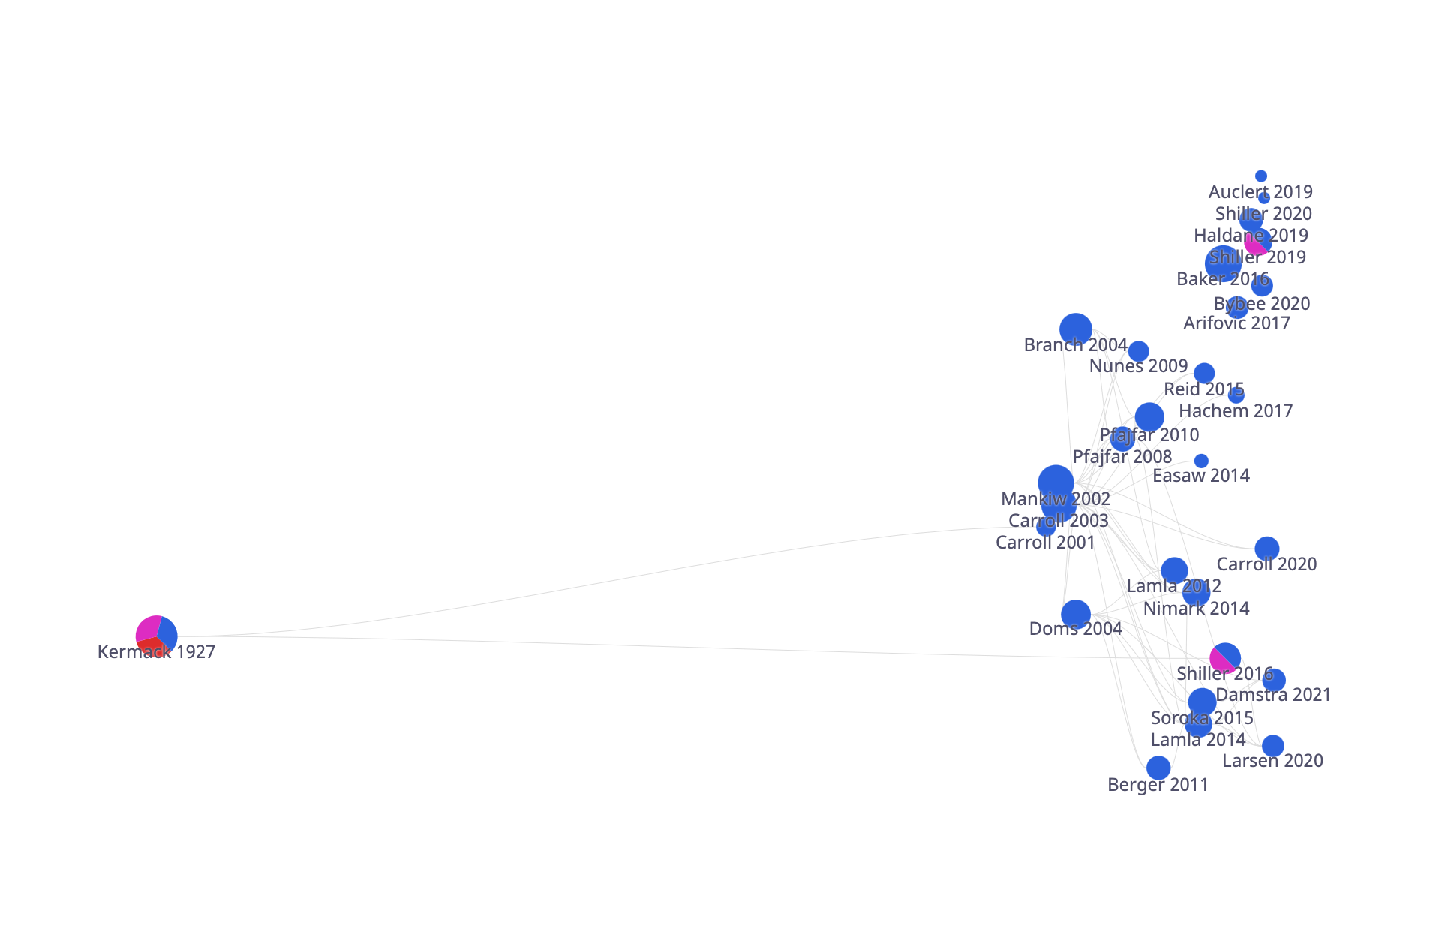
\includegraphics[width=1.5\textwidth]{./figures/graph_macro}}
	\begin{flushleft}
		{\footnotesize Note: This graph includes selected papers related to epidemiological models of macroeconomic expectations, and research on the interaction between news media and macroeconomic expectations. See \href{https://app.litmaps.co/shared/289F57F4-FDE5-4F94-B1A9-2BA7419DB719}{here} for its interactive version.}
	\end{flushleft}
\end{figure}


\subsubsection{Sticky Expectations}
%\noindent\textit{\textbf{Sticky Expectations of Inflation}}

%\noindent\cite{mr2002Sticky}-\cite{carroll2003macroeconomic}: Taken in combination, these two papers comprise a framework that satisfies our criteria of a full-fledged EE macroeconomic model -- though neither paper alone would qualify.

%\textit{Sticky Expectations.}

\cite{carroll2003macroeconomic} presents an epidemiological model in which the dynamics of aggregate consumer inflation expectations can be shown to follow a `sticky expectations' equation:
    \begin{align}
        M_{t}[\pi_{t+1}] & = (1-\lambda)M_{t-1}[\pi_{t}]+\lambda \mathbb{E}_{t}[\pi_{t+1}] \label{eq:StickyExp}
    \end{align}
where $M_{t}[\pi_{t+1}]$ reflects mean consumer expectations at date $t$ for inflation at date $t+1$, and $\mathbb{E}_{t}[\pi_{t+1}]$ is a `rational' expectation with which an individual consumer might be infected.

%\cite{carroll2003macroeconomic} fails the last of our criteria above for a full-bore EE macroeconomic model because he does not work out the consequences of the epidemiological model for macroeconomic dynamics, and \cite{mr2002Sticky} do not present an epidemiological model at all.  But \cite{carroll2003macroeconomic} is effectively an epidemiological microfoundation for \cite{mr2002Sticky}'s key expectational equation, which causes all the deviations of their results from a standard NK model.

%It may be useful here to sketch the key ingredients of the framework, to provide another fleshed-out example of how a simple epidemiological model can be constructed.

An analytical solution for aggregate dynamics of expectations is possible because the paper employs the simplest tool in the epidemiological toolkit: the common-source susceptible-infected (SI) model whose dynamics were traced out in table~\ref{table:SIDyn}.\footnote{See~\cite{easaw2015households} for a version that adds social learning between households.}   The idea is that consumers' expectations of inflation stem from exposure to (common) news media sources.  The elements of the framework are:
\begin{quote}
    \normalfont
\begin{enumerate}
    \item All news outlets report professional forecasters' consensus views\footnote{\cite{carroll2003macroeconomic} quotes news stories quoting professionals, and subsequent research by~\cite{lamla2014role} has confirmed the point.}
    \item Consumers and forecasters believe the same `true' inflation stochastic process
%    \begin{itemize}
%        \item It has purely transitory and purely permanent components
%        \item Shocks to those components are unpredictable
%    \end{itemize}
    \item All consumers are susceptible to infection with probability $\lambda$
    \item Infection means that the consumer adopts the view in the media
    \item The consumer retains that view until next infected
\end{enumerate}
\end{quote}

The consequence is a population distribution of beliefs in which a proportion of the population $(1-\lambda)^{n}$ holds the belief that was held by professional forecasters $n$ periods in the past.  Not only does this yield testable predictions about the distribution of beliefs in the microeconomic cross-section, it yields implications about the dynamics of the cross section, both of which are tested in the companion paper~\cite{carroll2001epidemiology}.  The possibility of testing a macroeconomic model using the dynamics of microeconomic cross-sectional expectations highlights a virtue of the approach:  measurable heterogeneity in expectations can provide a new kind of discipline for microfounded macroeconomic models.

The model was also constructed in the manner suggested in~Section~\ref{motivation-and-context}: It collapses to the rational expectations model as the parameter $\lambda$ approaches 1, so that it is straightforward to examine the consequences of the epidemiological deviation from RE.  In fact, the model can also be interpreted as nesting the `Rational Inattention' framework, to the extent that one further assumption seems plausible:  Beliefs about inflation derive from exposure to news coverage because the `reading the newspaper' method of becoming informed is almost infinitely easier than solving (yourself) the full-fledged Rational Inattention macroeconomic model.\footnote{It is more plausible to model the professional forecasters themselves as having the skills and time and motivation to solve the full Rational Inattention model - or, alternatively, an EE model.}

Another implication that flows from the model -- inflation expectations are a result of the degree of exposure to news stories -- leads to a straightforward implication:  The speed at which inflation expectations move toward the rational expectation will depend on the intensity of news coverage of inflation.  \cite{carroll2003macroeconomic} found some support for this implication; \cite{lamla2014role} and \cite{larsen2021news} find further evidence that greater intensity of news coverage of inflation leads to more accurate expectations in the population.  % CDC: we should cite this:  More recently,  identified topics discussed in the news media related to inflation using machine learning algorithms and found they are good predictions of inflation expectations. The intensity of inflation-related topics in the news media accounts for the time-varying rigidity in information, as predicted in the model.

%% CDC: We some how do not have doms et al's paper on sentiment now. We should include it.  \cite{doms2004consumer} .

%\footnote{See \cite{}, and in particular the clever paper by doms et al which}.

% For slides: These results may be of some interest at the present moment when news coverage about inflation is intense.  But another result from the paper is also interesting: An explicit horserace was done between a version of the model in which consumers' views adjusted toward the most recently reported actual inflation statistic, versus adjusting toward professional forecasters predictions of future inflation.

%\noindent\textit{Sticky Information.}

In a paper written independently of and published before \cite{carroll2003macroeconomic}, \cite{mr2002Sticky} simply assume that the dynamics of inflation expectations are given by a process like \eqref{eq:StickyExp}; they call this a `sticky information' assumption,\footnote{See \bvbayesianlearningFull for a potential microfoundation.} and argue that the macroeconomic implications of a New Keynesian model in which expectations work this way match a variety of facts (most notably, the sluggishness of inflation dynamics) that standard NK models cannot capture.

The combination of their paper with that of~\cite{carroll2003macroeconomic} is closer to constituting a full-fledged EE approach to macroeconomic modeling than either paper is alone: Carroll's paper did not examine the consequences of his model of inflation expectations for anything else, while \cite{mr2002Sticky} did not provide an epidemiological motivation for their `sticky information' equation.  (Conveniently, however, their baseline calibration of the model was to set $\lambda=0.25$, while Carroll's empirical estimate of the parameter was $0.27$.)\footnote{A number of subsequent papers have estimated similar equations in a variety of countries, generally finding roughly similar results.}

\cite{mankiw2007sticky} extend the analysis of their earlier paper to a general equilibrium context with goods, labor, and financial markets, and point out explicitly that the stickiness that drives the core results in their new model can be motivated by an epidemiological model.

\subsubsection{Effectiveness of Monetary Policy}

Heterogeneous expectations have important implications for the effectiveness of central bank communication.   To capture this point, \cite{hachem_inflation_2017} construct a model in which monopolistically competitive firms hold heterogeneous inflation expectations due to different forecasting rules. One group of firms simply expect inflation to remain stable (``Random Walkers''), and the other group makes forecasts based on central bank announcements (``Fed Watchers''). The fraction of Fed Watchers summarizes the credibility of the central bank.  The model's epidemiological content comes from the transmission of beliefs about which strategies to pursue:  firms meet each other and potentially switch forecasting rules based on relative performance. The paper shows that for the central bank, a period of gradual announcements helps build credibility and achieves target inflation, while an abrupt change in the target leads to undershooting.

\subsubsection{Sticky Consumption}

A number of recent papers including \cite{carroll2020sticky} and \cite{auclert2020micro} have applied the same epidemiological model used in \cite{carroll2003macroeconomic} to the problem of consumers whose attention to the macroeconomic news relevant for their consumption decisions may be spotty even if they are very well informed about their own idiosyncratic circumstances.  The consequence turns out to be that aggregate consumption exhibits `excess smoothness' in a way that matches data dynamics well, while at the same time predictions about microeconomic behavior are consistent with the micro facts that have been used to discipline the new generation of HA-Macro models.

%One advantage of the consumption context over that of inflation is that consumers have a utility function that can be used to calculate the cost of deviations from instantaneous and perfect updating.  When the `news infectiousness' parameter is calibrated so that the model's consumption dynamics match aggregate consumption dynamics, the cost to consumers of failing to read every news story (alternatively, of the `infectiousness' of news being less than 100 percent) is negligible.  This is because the vast majority of the uncertainty consumers face stems from idiosyncratic, not aggregate, risks, so being a little bit out of date with respect to the latest aggregate developments has only a very small cost.

\subsubsection{Social Learning of Macroeconomic Equilibria}

As we noted earlier, many approaches to economic questions can be described using the language of epidemiological modeling even though that terminology is not how the authors described their own work.  This is true, for example, of work on ``social learning'' in macroeconomics.  For example, in \cite{arifovic2018learning}, an economy with agents who have different macroeconomic forecasting rules evolves as agents discard their own rules when they encounter others whose rules have proven more effective.  Another way of describing this process would be to say that the more effective rules are more infectious.  Indeed, the parallel to the biological process is deeper: As diseases can do, the rules can mutate into more (or less) effective forms.  The paper also discusses the potential role of professional forecasters and the extent to which their views can spread to the population at large -- in our terminology, because their views are more `viral.'

\cite{tesfatsion2006agent} has made a sustained case that agent based modeling has application to many subfields of economics, but it seems likely that almost all of that literature could also be reinterpreted as being about the transmission of expectations (when it is not already explicitly formulated in those terms, as in~\cite{hommes2006heterogeneous}).  An example closely related to the explicitly epidemiological work on inflation expectations is \cite{branchHeteroExp}, who considers a model in which agents with different inflation forecasting rules compete and the rules that work better are adopted.  \cite{haldane_drawing_2019} make a strong case for a broad interpretation (or reinterpretation) of these kinds of models as epidemiological, particularly in the macroeconomic context.  As with the work on agent based modeling in finance, we chose not to attempt a summary of this literature because excellent comprehensive surveys already exist (see, e.g., \cite{ddAgentBasedMacro}), and because little of the literature focuses explicitly on the dynamics of measured expectations.  But readers interested in these subjects would do well to absorb this work (and especially the work of Hommes).

\begin{comment}
\subsubsection{Other Work}

Among our criteria for narrowing the scope of what constitutes a `full-fledged' EE modeling approach, the most effective was our requirement that the expectation dynamic have a clear connection to some separately measurable economic outcome.

Because expectations of inflation (or of other variables) are so widely believed (by economists, at least) to be a driver of actual inflation outcomes, we have permitted ourselves to include models that measure themselves by their success in explaining the movements in surveyed expectations.

But that leap does require belief in a connection between measured beliefs and actual choices

One question that might arise is whether news coverage is a plausible driver of actual consumer behavior.  Several papers have found evidence that news coverage does have substantial impact on households' beliefs about economic matters.  A clever paper by \cite{doms2004consumer} shows that consumer sentiment is driven by news coverage even during periods in which coverage is inconsistent with economic conditions.  (They cite an extensive prior literature that has found evidence that consumer sentiment itself is correlated with economic choices in ways not captured by other observable macroeconomic variables).\footnote{For further evidence that news coverage is a key source of people's views, see \cite{lamla2012role}, though see~\cite{pfajfar2013news} for a skeptical view.  }


\begin{itemize}
	\item \cite{carroll2003macroeconomic}, \href{http://www.econ2.jhu.edu/people/ccarroll/epidemiologySFI.pdf}{\cite{carroll2005epidemiology}}: ``rational'' forecasts by professionals spread to average households as in a common source epi model
	\begin{itemize}
		\item insights:  arguably simplest model that could be interpreted as ``epidemiological''
		\item mechanism:
		\begin{itemize}
			\item
			ordinary people: exposed, at constant rate, to news media which reports what ``experts'' say
			\item
			fraction of people who absorb those views depends on ``infectiousness'' of experts' views
			\item $\Rightarrow$ population beliefs are geometric lag of experts' beliefs
			\item
			embeds RE model as the limit corresponding to ``infinitely instantly
			perfectly infectious'' beliefs
		\end{itemize}
		\item implications:
		\begin{itemize}
			\item
			stickiness of aggregate expectations: most recent economic news \href{http://www.econ2.jhu.edu/people/ccarroll/epidemiologySFI.pdf}{\cite{carroll2005epidemiology}}, \href{http://www.econ2.jhu.edu/people/ccarroll/epidemiologyQJE.pdf}{\cite{carroll2003macroeconomic}} and policy annoucements  \href{https://www.tcd.ie/Economics/staff/waltis/EC2010/ec2010_ps5ans.pdf}{\cite{berger2011monetary}} do not reach to all private agents instantaneously
			\item aggregated sluggishness in adjustment in shock responses, i.e. consumption \href{https://www.ecb.europa.eu/pub/pdf/scpwps/ecb.wp2152.en.pdf}{\cite{carroll2020sticky}},  \href{https://www.nber.org/papers/w26647}{\cite{auclert2020micro}};
			\item
			which affects what Fed governors and treasury secretaries do, e.g. central bank communication
		\end{itemize}
	\end{itemize}

	\item \cite{doms2004consumer}:  consumer sentiment driven by news coverage even during periods in which news coverage is inconsistent with economic conditions.
	\item \href{https://github.com/iworld1991/EpiExp/blob/master/Literature/lamla2012role.pdf}{\cite{lamla2012role}}: disagreement of households depends on the heterogeneity of story contentand on the reporting intensity, especially of news on rising inflation. Disagreement of professional forecasters does not depend on media coverage. % MICHAEL J. LAMLA THOMAS MAAG The Role of Media for Inflation Forecast Disagreement of Households and Professional Forecasters This paper investigates the effects of media coverage about consumer price inflation on inflation forecast disagreement of German households and pro-fessional forecasters. We adopt a Bayesian learning model in which mediacoverage of inflation affects forecast disagreement by influencing infor-mation sets as well as predictor choice. Our empirical results show that disagreement of households depends on the heterogeneity of story contentand on the reporting intensity, especially of news on rising inflation. Dis-agreement of professional forecasters does not depend on media coverage.With respect to the influence of macroeconomic variables, we provide ev-idence that disagreement of professional forecasters primarily depends onthe inflation rate and on inflation volatility. The response of households toinflation is much less pronounced.
	\item \href{https://github.com/iworld1991/EpiExp/blob/master/Literature/pfajfar_news_2013.pdf}{\cite{pfajfar_news_2013}}: tests the epidemiological model using directly reported news exposure in the Michigan Survey(``news heard about aggregate price changes''(available since 1961)) and finds that recent news exposure does not lead to more accurate forecasts. Most of the households seem to not adjust beliefs toward recent professional forecasts. The authors attribute this to distorted information reported in the news in the first place.    %Specifically, the following question is addressed to each household "During the last few months, have you heard of any favorable or unfain business conditions?"12 In case of an affirmative response, a second question is asked: "What did you hear?" To address this query, the respondent is presented with a number of options regarding the type of business conditions she might have heard about, such as government, unemployment, prices, consumer demand, stock market, credit, and trade deficit. She is allowed to name at most two of these options. Should prices be one of the selected options, she can reply either (i) "Favorable News: Lower Prices" or (ii) "Unfavorable News: Higher Prices.

	%"Moreover, it appears that households do not make the best use of the information they perceive, as they persistently deviate from professional forecasters' mean expectation, displaying no tendency to adjust their forecasts appropriat. One possible interpretation is that news transmitted by the media distorts consumers' expectations, as it may contain judgmental assess ments of professional forecasters' views. As a consequence, media reports could be biased and the epidemiological mechanism results as a channel that transmits dis torted expectations. This factor could also explain why the degree of perception of unfavorable news on prices is significantly higher than that of favorable news, and why the accuracy of consumers' expectations decreases in the volume of negative news being perceiv"
	% A link to michigan survey on news heard about prices https://data.sca.isr.umich.edu/get-chart.php?y=2021&m=1&n=23h&d=ylch&f=pdf&k=ce35d9fed5ce19c35c089331bd03e10e68f96c690f6bac22c6a77be0beda6204

	\item \href{http://www.sarah-lein.ch/pdfs/inflationexpectations.pdf}{\cite{lamla2014role}}:  the intensity of media reporting of inflation leads to forecast accuracy while the content may bias the inflation expectations.  It augments \cite{carroll2003macroeconomic} with Bayesian learning at individual level admitting bias from the media. %This paper analyzes the impact of the media on consumers’ inflation expectations. We distinguish between two channels through which the media can influence expectations. First, the intensity of the coverage of inflation reports plays a role (volume channel). Second, the content of media reports have an effect (tone channel). Employing a detailed data set capturing media reports on inflation in Germany during the period comprising 01/1998-09/2007, we are able to discriminate between these two effects. We find that the volume effect improves the accuracy of consumers’ forecasts, whereas the tone channel may bias inflation expectations
	\item \href{https://github.com/iworld1991/EpiExp/blob/master/Literature/hachem_inflation_2017.pdf}{\cite{hachem_inflation_2017}}:  the effectiveness of central bank announcements when firms have heterogeneous inflation expectations a la \cite{carroll2003macroeconomic}.
	\item These work suggest that the canonical common-source epidemiological model can be enriched to be reflect the differences in the sources of the infection(news media, professional forecasts, or statistical agencies, etc) and the belief updating rule by households(Bayesian signal extraction or naive updating, etc) can be useful to match macroeconomic expectation dynamics.
\end{itemize}

\end{comment}
